\section{Release notes}

%\begin{equation}
%\sum\limits_{i=1}^n i^2 = \frac{n(n+1)(2n+1)}{6}
%\end{equation}

\subsection{Adaptations to the astrocyte model}
In the creation of NVU 1.1 the work of Farr\& David(2011) \cite{Farr2011} was implemented in NVU 1.0. This means that several pathways were added and equations were combined. First a glutamate release in the synaptic cleft was simulated by creating a smooth pulse function, $\rho$, describing the ratio of bound to total glutamate receptors on the synapse end of the astrocyte. This induces an \gls{IP3} release into the cell, causing the release of Calcium from the \gls{ER} into the cytosol, which on his turn leads to the production of EET. The open state of the BK-channels in NVU 1.0 depends only on the membrane voltage, in NVU 1.1 the opening of BK-channels is regulated by the membrane voltage as well as the EET and \gls{Ca} concentration. Furthermore, several corrections, proposed by de Kock \& van der Donck (2013) \cite{LoesEvert}, on the model by Farr were included. These corrections include an equation to describe the buffering parameter in the \gls{Ca} conservation equation (Farr \cite{Farr2011} used a constant to describe this parameter) and some changes in parameter values.


\subsection{New/changed equations \& parameters for the astrocyte model}
\paragraph{$\rho$ input signal}

The smooth pulse function $\rho$
\begin{equation}
\rho(t) = \frac{Amp - base}{2}\times\left(1+\mathrm{tanh}\left(\frac{t-t_0}{\theta_L}\right)\right)+base+\frac{Amp-base}{2}\times\left(1+\mathrm{tanh}\left(\frac{t-t_2}{\theta_R}\right)\right)+base-Amp     
\end{equation}
%
\begin{table}[h!]
	\centering
	\begin{tabular}{| p{0.09\linewidth} | >{\footnotesize} p{0.6\linewidth} | >{\footnotesize} p{0.17\linewidth} | >{\footnotesize} p{0.02\linewidth} |}
		\arrayrulecolor{lightgrey}\hline
		$Amp$           & Amplitude of smooth pulse function & 0.5 & ME\\
		$base$          & Baseline of smooth pulse function & 0.1 & ME\\
		$\theta_L$      & Left ramp of smooth pulse function & 1 & ME\\
		$\theta_R$      & Left ramp of smooth pulse function & 1 & ME\\
		\hline
	\end{tabular}
\end{table}

\subsubsection{Conservation Equations}
\gls{Ca} concentration in the astrocytic cytosol:
\begin{equation} \label{eqRN:ckInt}
\dfrac{\mathrm{d}c_k}{\mathrm{d}t}= B_{\mathrm{cyt}}(J_{\mathrm{IP_3}}-J_{\mathrm{pump}}+J_{\mathrm{ER_leak}})
\end{equation}
%
\gls{Ca} concentration in the astrocytic \gls{ER}:
\begin{equation} \label{eqRN:skInt}
\dfrac{\mathrm{d}s_k}{\mathrm{d}t}= \frac{1}{VR_{\mathrm{ER_cyt}}}(\frac{dc_k}{dt})
\end{equation}
%
The inactivation variable for \gls{IP3}:
\begin{equation} \label{eqRN:hkInt}
\dfrac{\mathrm{d}h_k}{\mathrm{d}t}= k_{\mathrm{on}}[K_{\mathrm{inh}}-(c_k+K_{\mathrm{inh}})h_k]
\end{equation}
%
The \gls{IP3} concentration:
\begin{equation} \label{eqRN:ikInt}
\dfrac{\mathrm{d}i_k}{\mathrm{d}t}= r_hG-k_{\mathrm{deg}}i_k
\end{equation}
%
The EET concentration:
\begin{equation} \label{eqRN:eetkInt}
\dfrac{\mathrm{d}eetk_k}{\mathrm{d}t}= V_{\mathrm{eet}}(c_k-c_{\mathrm{k,min}})-k_{\mathrm{eet}}eet_k
\end{equation}
%
Open probability of the BK channel (\pers):
\begin{equation} \label{eqRN:dwkdt}
\frac{\mathrm{d}w_{k}}{\mathrm{d}t} = \phi_{w} \left(w_{\infty}-w_{k} \right) 
\end{equation}

\begin{table}[h!]
	\centering
	\begin{tabular}{| p{0.09\linewidth} | >{\footnotesize} p{0.6\linewidth} | >{\footnotesize} p{0.17\linewidth} | >{\footnotesize} p{0.02\linewidth} |}
		\arrayrulecolor{lightgrey}\hline
		$ VR_{\mathrm{ER_{\mathrm{cyt}}}} $  & Volume ratio of the \gls{ER} to the cytosol in the astrocyte  & 0.185 [-] & \cite{Farr2011} \\
		$k_{\mathrm{on}} $         & Rate of \gls{Ca} binding to the \gls{IP3}R & 2 [\uMps] & \cite{Farr2011} \\
		$K_{\mathrm{inh}}$          & Dissociation rate of $k_{\mathrm{on}}$  & [0.1\uM] & \cite{Farr2011} \\
		$r_h$                      & Maximum rate of \gls{IP3} production in the astrocyte & 4.8 [\uM] & \cite{Farr2011} \\
		$k_{\mathrm{deg}}$          & Rate constant for \gls{IP3} degradation & 1.25 [\pers] & \cite{Farr2011} \\
		$V_{\mathrm{eet}} $        & Rate constant for EET production   & 72[\uM] & \cite{Farr2011} \\
		$k_{\mathrm{eet}}$         & Rate constant for EET degradation  & 7.2[\uM] & \cite{Farr2011} \\
		$c_{\mathrm{k,min}}$       & Minimum \gls{Ca} concentration required for EET production & 0.1 [uM] & \cite{Farr2011} \\			
		\hline
	\end{tabular}
\end{table}
		
\subsubsection{Fluxes}
\gls{Ca} flux from the ER to the cytosol in the astrocyte through \gls{IP3} Receptors (\gls{IP3}R) by \gls{IP3}: 
\begin{equation} \label{eqRN:J_ip3}
J_{\mathrm{IP3}}=J_{\mathrm{max}}[(\frac{i_k}{i_k+K_i})(\frac{c_k}{c_k+K_{\mathrm{act}}})h_k]^3\times [1-\frac{c_k}{s_k}] 
\end{equation}
%
The leakage \gls{Ca}  flux from the \gls{ER} to the cytosol in the astrocyte:
\begin{equation} \label{eqRN:J_ER_leak}
J_{\mathrm{ER_leak}} = P_L(1-\frac{c_k}{s_k})
\end{equation}	
%
The ATP dependent \gls{Ca}  pump flux from the cytoplasm to the ER in the astrocyte:
\begin{equation} \label{eqRN:J_pump}
J_{\mathrm{pump}} = V_{\mathrm{max}}\frac{c_k^2}{c_k^2+k_pump^2}
\end{equation}
\begin{table}[h!]
	\centering
	\begin{tabular}{| p{0.09\linewidth} | >{\footnotesize} p{0.6\linewidth} | >{\footnotesize} p{0.17\linewidth} | >{\footnotesize} p{0.02\linewidth} |}
		\arrayrulecolor{lightgrey}\hline	
		$J_{max}$       & Maximum \gls{IP3} rate                                                & 2880 \uMps        & \cite{Farr2011} \\  
		$K_I$           & Dissociation constant for \gls{IP3} binding to \gls{IP3}R             & 0.03 \uM          & \cite{Farr2011} \\ 
		$K_{act}$       & Dissociation constant for \gls{Ca} binding to \gls{IP3}R              & 0.17 \uM          & \cite{Farr2011} \\ 
		$P_L$           & Associated with the steady state \gls{Ca} balance                     & 0.0842 \uM           & \cite{LoesEvert} \\ 
		$V_{max}$       & Maximal pumping rate of the \gls{Ca} pump                             & 20 \uMps          & \cite{Farr2011} \\ 
		$k_{pump}$      & Dissociation constant of the \gls{Ca} pump                            & 0.24 \uM          & \cite{Farr2011} \\ 
		\hline
	\end{tabular}
\end{table}
\subsubsection{Additional equations}
The Calcium buffering parameter in the astrocytic cytosol (-)
\begin{equation} \label{eqRN:B_cyt}
B_{cyt}=\left(1+BK_{end}+ \frac{K_{ex}B_{ex}}{(K_{ex}+c_k)^2}\right)^{-1} 
\end{equation}
The ratio of active to total G-protein (-)
\begin{equation} \label{eqRN:G}
G=\frac{\rho+\delta}{K_g+\rho+\delta}
\end{equation}
Equilibrium state BK-channel (-):
\begin{equation} \label{eqRN:winf}
w_{\infty}=0.5 \left(1+\mathrm{tanh}\left(\frac{v_{k}+(eet_{\mathrm{shift}}eet_k)-v_{3} }{v_{4}} \right)  \right) 
\end{equation}
%
The time constant associated with the opening of BK channels	 (in \pers):
\begin{equation} \label{eqRN:phin}
\phi_{w}=\psi_{w}\mathrm{cosh}\left( \frac{v_{k}-v_{3}}{2v_{4}}\right) 
\end{equation}
\gls{Ca} dependent shift of the opening of the BK-channels
\begin{equation} \label{eqRN:v_3}
v_{3}=\frac{v_5}{2}\mathrm{tanh}\left( \frac{c_k-Ca_3}{Ca_4}\right)+v_6 
\end{equation}

\begin{table}[h!]
	\centering
	\begin{tabular}{| p{0.09\linewidth} | >{\footnotesize} p{0.6\linewidth} | >{\footnotesize} p{0.17\linewidth} | >{\footnotesize} p{0.02\linewidth} |}
		\arrayrulecolor{lightgrey}\hline
		
		$BK_{end}$      & Cytosolic endogenous buffer constant                              & 40 [-] & \cite{LoesEvert} \\
		$K_{ex}$        & Cytosolic exogenous buffer dissociation constant                  & 0.26 [\uM] & \cite{LoesEvert} \\
		$B_{ex}$        & Concentration of cytosolic exogenous buffer                       & 11.35 [\uM] & \cite{LoesEvert} \\
		$\delta$        & Ratio of the activities of the bound and unbound receptors        & 1.235e-3 [-] & \cite{Farr2011}\\
		$K_G$           & The G-protein dissociation constant                               & 8.82  [-] & \cite{Farr2011}\\
		$v_{4}$			& A measure of the spread of the distribution of the open probability of the BK channel	& 14.5e-3 [\Volt]   &  \cite{Gonzalez1994} \\
		$v_{5}$			& Determines the range of the shift of $n_{\inf}$ as calcium varies    	& 8e-3 [\Volt]  & \cite{Farr2011}  \\
		$v_{6}$			& The voltage associated with the opening of half the population		& -15e-3 [\Volt]  & \cite{Farr2011}  \\
		$ \psi_{w}$    	& A characteristic time for the open probability of the BK channel		& 2.664 [$s^{-1}$] & \cite{Gonzalez1994} \\
		
		\hline
	\end{tabular}
\end{table}

\subsection{Corrections}
A mistake was discovered in NVU1.0 for the equation used to describe the \gls{K} concentration in the synaptic cleft. The original equation subtracted the change in astrocytic \gls{K} concentration from the \gls{K} influx from the neuron. This was incorrect since not all channels lead from the astrocyte to the synaptic cleft. The BK-channel describes the flux from the astrocyte to the perivascular space, and therefore this flux was added to the equation, resulting in (\ref{eq:KEx}). Fortunately this mistake led to very small changes, and it did not significantly change the model outcomes. Figure \ref{fig:cordif} shows the old and the corrected results for the flux through the BK-channel, and it is clear that they practically overlap. 

\begin{figure}[h!]
	\centering
	\tiny 
%				\newlength\figureheight 
%				\newlength\figurewidth 
	\setlength\figureheight{5 cm} 
	\setlength\figurewidth{15 cm}
%	% This file was created by matlab2tikz v0.3.3.
% Copyright (c) 2008--2013, Nico Schlömer <nico.schloemer@gmail.com>
% All rights reserved.
% 
% The latest updates can be retrieved from
%   http://www.mathworks.com/matlabcentral/fileexchange/22022-matlab2tikz
% where you can also make suggestions and rate matlab2tikz.
% 
% 
% 
\begin{tikzpicture}

\begin{axis}[%
width=\figurewidth,
height=\figureheight,
scale only axis,
xmin=0,
xmax=500,
ymin=-1.5e-07,
ymax=3e-07
]
\addplot [
color=blue,
solid,
forget plot
]
table[row sep=crcr]{
0 6.9104e-09\\
0.00089136 6.8832e-09\\
0.0017827 6.8977e-09\\
0.0026741 6.9081e-09\\
0.0061751 6.946e-09\\
0.0096762 6.9813e-09\\
0.013177 7.0146e-09\\
0.016678 7.0457e-09\\
0.026472 7.1229e-09\\
0.036266 7.1874e-09\\
0.04606 7.2413e-09\\
0.055854 7.2861e-09\\
0.065648 7.3232e-09\\
0.075699 7.3541e-09\\
0.079199 7.3634e-09\\
0.0827 7.372e-09\\
0.086201 7.3799e-09\\
0.089702 7.3871e-09\\
0.093202 7.3936e-09\\
0.10095 7.4061e-09\\
0.1087 7.4159e-09\\
0.11645 7.4232e-09\\
0.12421 7.4283e-09\\
0.14151 7.4325e-09\\
0.15881 7.4284e-09\\
0.17612 7.4176e-09\\
0.19342 7.4014e-09\\
0.21073 7.3808e-09\\
0.2497 7.3221e-09\\
0.28868 7.2524e-09\\
0.32765 7.1764e-09\\
0.36662 7.097e-09\\
0.37628 7.077e-09\\
0.38594 7.0569e-09\\
0.39561 7.0367e-09\\
0.40527 7.0164e-09\\
0.41493 6.9961e-09\\
0.43002 6.9643e-09\\
0.44221 6.9385e-09\\
0.4544 6.9127e-09\\
0.46659 6.8869e-09\\
0.47879 6.8611e-09\\
0.49098 6.8353e-09\\
0.51139 6.7921e-09\\
0.52695 6.7592e-09\\
0.54251 6.7264e-09\\
0.55807 6.6937e-09\\
0.57363 6.6611e-09\\
0.58919 6.6286e-09\\
0.6088 6.5878e-09\\
0.6284 6.5472e-09\\
0.64801 6.5067e-09\\
0.66761 6.4665e-09\\
0.68722 6.4265e-09\\
0.73766 6.3247e-09\\
0.78811 6.2244e-09\\
0.83855 6.1257e-09\\
0.889 6.0286e-09\\
0.93944 5.9331e-09\\
1.0031 5.815e-09\\
1.0667 5.6994e-09\\
1.1303 5.5863e-09\\
1.1939 5.4757e-09\\
1.2576 5.3675e-09\\
1.3769 5.171e-09\\
1.4783 5.0103e-09\\
1.5797 4.8552e-09\\
1.6811 4.7054e-09\\
1.7825 4.5608e-09\\
1.8839 4.4211e-09\\
2.0684 4.1791e-09\\
2.2528 3.9516e-09\\
2.4373 3.7376e-09\\
2.6218 3.5362e-09\\
2.8063 3.3464e-09\\
2.9907 3.1676e-09\\
3.3424 2.8543e-09\\
3.694 2.5735e-09\\
4.0456 2.3213e-09\\
4.3972 2.0943e-09\\
4.7489 1.8898e-09\\
5.2238 1.645e-09\\
5.6986 1.4315e-09\\
6.1735 1.245e-09\\
6.6484 1.0817e-09\\
7.1233 9.387e-10\\
7.8241 7.5915e-10\\
8.525 6.1081e-10\\
9.2258 4.8795e-10\\
9.9266 3.8599e-10\\
10.627 3.012e-10\\
11.627 2.0422e-10\\
12.627 1.2907e-10\\
13.627 7.0379e-11\\
14.627 2.4167e-11\\
15.627 -1.2598e-11\\
16.627 -4.2229e-11\\
17.627 -6.6506e-11\\
18.627 -8.6869e-11\\
19.627 -1.0426e-10\\
20.627 -1.1939e-10\\
21.627 -1.3282e-10\\
22.627 -1.4491e-10\\
23.627 -1.5597e-10\\
24.627 -1.6623e-10\\
25.627 -1.7585e-10\\
26.627 -1.8489e-10\\
27.627 -1.9342e-10\\
28.627 -2.0149e-10\\
29.627 -2.0914e-10\\
30.627 -2.1638e-10\\
31.627 -2.2325e-10\\
32.627 -2.2975e-10\\
33.627 -2.359e-10\\
34.627 -2.4174e-10\\
35.627 -2.4727e-10\\
36.627 -2.5251e-10\\
37.627 -2.5748e-10\\
38.627 -2.6219e-10\\
39.627 -2.6664e-10\\
40.627 -2.7084e-10\\
41.627 -2.7474e-10\\
42.627 -2.7831e-10\\
43.627 -2.8149e-10\\
44.627 -2.8421e-10\\
45.627 -2.864e-10\\
46.627 -2.88e-10\\
47.627 -2.89e-10\\
48.627 -2.8941e-10\\
49.627 -2.8932e-10\\
50.627 -2.8882e-10\\
51.627 -2.8805e-10\\
52.627 -2.8713e-10\\
53.627 -2.8617e-10\\
54.627 -2.8527e-10\\
55.627 -2.8448e-10\\
56.627 -2.8384e-10\\
57.627 -2.8336e-10\\
58.627 -2.8304e-10\\
59.627 -2.8287e-10\\
60.627 -2.8283e-10\\
61.627 -2.829e-10\\
62.627 -2.8306e-10\\
63.627 -2.8329e-10\\
64.627 -2.8357e-10\\
65.627 -2.8388e-10\\
66.627 -2.842e-10\\
67.627 -2.8452e-10\\
68.627 -2.8483e-10\\
69.627 -2.851e-10\\
70.627 -2.8535e-10\\
71.627 -2.8555e-10\\
72.627 -2.8571e-10\\
73.627 -2.8582e-10\\
74.627 -2.8589e-10\\
75.627 -2.8593e-10\\
76.627 -2.8592e-10\\
77.627 -2.859e-10\\
78.627 -2.8585e-10\\
79.627 -2.8578e-10\\
80.627 -2.8571e-10\\
81.627 -2.8564e-10\\
82.627 -2.8556e-10\\
83.627 -2.855e-10\\
84.627 -2.8544e-10\\
85.627 -2.8539e-10\\
86.627 -2.8536e-10\\
87.627 -2.8534e-10\\
88.627 -2.8533e-10\\
89.627 -2.8532e-10\\
90.627 -2.8533e-10\\
91.627 -2.8535e-10\\
92.627 -2.8537e-10\\
93.627 -2.8539e-10\\
94.627 -2.8542e-10\\
95.627 -2.8544e-10\\
96.627 -2.8546e-10\\
97.627 -2.8549e-10\\
98.627 -2.855e-10\\
99.627 -2.8552e-10\\
100.63 -2.8553e-10\\
101.63 -2.8554e-10\\
102.63 -2.8555e-10\\
103.63 -2.8555e-10\\
104.63 -2.8555e-10\\
105.63 -2.8555e-10\\
106.63 -2.8555e-10\\
107.63 -2.8554e-10\\
108.63 -2.8554e-10\\
109.63 -2.8554e-10\\
110.63 -2.8553e-10\\
111.63 -2.8553e-10\\
112.63 -2.8552e-10\\
113.63 -2.8552e-10\\
114.63 -2.8552e-10\\
115.63 -2.8551e-10\\
116.63 -2.8551e-10\\
117.63 -2.8551e-10\\
118.63 -2.8551e-10\\
119.63 -2.8551e-10\\
120.63 -2.8551e-10\\
121.63 -2.8551e-10\\
122.63 -2.8551e-10\\
123.63 -2.8551e-10\\
124.63 -2.8552e-10\\
125.63 -2.8552e-10\\
126.63 -2.8552e-10\\
127.63 -2.8552e-10\\
128.63 -2.8552e-10\\
129.63 -2.8552e-10\\
130.63 -2.8552e-10\\
131.63 -2.8552e-10\\
132.63 -2.8552e-10\\
133.63 -2.8552e-10\\
134.63 -2.8552e-10\\
135.63 -2.8552e-10\\
136.63 -2.8552e-10\\
137.63 -2.8552e-10\\
138.63 -2.8552e-10\\
139.63 -2.8552e-10\\
140.63 -2.8552e-10\\
141.63 -2.8552e-10\\
142.63 -2.8552e-10\\
143.63 -2.8552e-10\\
144.63 -2.8552e-10\\
145.63 -2.8552e-10\\
146.63 -2.8552e-10\\
147.63 -2.8552e-10\\
148.63 -2.8552e-10\\
149.63 -2.8552e-10\\
150.63 -2.8552e-10\\
151.63 -2.8552e-10\\
152.63 -2.8552e-10\\
153.63 -2.8552e-10\\
154.63 -2.8552e-10\\
155.63 -2.8552e-10\\
156.63 -2.8552e-10\\
157.63 -2.8552e-10\\
158.63 -2.8552e-10\\
159.63 -2.8552e-10\\
160.63 -2.8552e-10\\
161.63 -2.8552e-10\\
162.63 -2.8552e-10\\
163.63 -2.8552e-10\\
164.63 -2.8552e-10\\
165.63 -2.8552e-10\\
166.63 -2.8552e-10\\
167.63 -2.8552e-10\\
168.63 -2.8552e-10\\
169.63 -2.8552e-10\\
170.63 -2.8552e-10\\
171.63 -2.8552e-10\\
172.63 -2.8552e-10\\
173.63 -2.8552e-10\\
174.63 -2.8552e-10\\
175.63 -2.8552e-10\\
176.63 -2.8552e-10\\
177.63 -2.8552e-10\\
178.63 -2.8552e-10\\
179.63 -2.8552e-10\\
180.63 -2.8552e-10\\
181.63 -2.8552e-10\\
182.63 -2.8552e-10\\
183.63 -2.8552e-10\\
184.63 -2.8552e-10\\
185.63 -2.8552e-10\\
186.63 -2.8552e-10\\
187.63 -2.8552e-10\\
188.63 -2.8552e-10\\
189.63 -2.8552e-10\\
190.63 -2.8552e-10\\
191.63 -2.8552e-10\\
192.63 -2.8552e-10\\
193.63 -2.8552e-10\\
194.63 -2.8552e-10\\
195.63 -2.8552e-10\\
196.63 -2.8552e-10\\
197.19 -2.8552e-10\\
197.62 -2.8552e-10\\
197.92 -2.8552e-10\\
198.17 -2.8552e-10\\
198.37 -2.8552e-10\\
198.57 -2.8552e-10\\
198.71 -2.8552e-10\\
198.85 -2.8552e-10\\
198.97 -2.8552e-10\\
199.09 -2.8552e-10\\
199.21 -2.8552e-10\\
199.4 -2.8552e-10\\
199.6 -2.8552e-10\\
199.8 -2.8552e-10\\
199.99 -2.8552e-10\\
200.31 2.4767e-09\\
200.54 8.1536e-09\\
200.77 1.7782e-08\\
201.01 3.1713e-08\\
201.24 5.0205e-08\\
201.54 8.0989e-08\\
201.84 1.1947e-07\\
202.14 1.6234e-07\\
202.43 2.022e-07\\
202.73 2.3092e-07\\
203.03 2.4288e-07\\
203.33 2.3577e-07\\
203.42 2.3001e-07\\
203.51 2.227e-07\\
203.6 2.1407e-07\\
203.69 2.0435e-07\\
203.78 1.9372e-07\\
203.89 1.7916e-07\\
204 1.6373e-07\\
204.12 1.4772e-07\\
204.23 1.3136e-07\\
204.34 1.1491e-07\\
204.53 8.8799e-08\\
204.71 6.3643e-08\\
204.89 3.9996e-08\\
205.08 1.8254e-08\\
205.45 -1.9481e-08\\
205.83 -4.6844e-08\\
206.2 -6.3799e-08\\
206.58 -7.1719e-08\\
207.23 -7.0233e-08\\
207.87 -5.9441e-08\\
208.52 -4.6614e-08\\
209.17 -3.5115e-08\\
209.82 -2.6255e-08\\
210.52 -1.9077e-08\\
211.23 -1.3747e-08\\
211.93 -1.0168e-08\\
212.64 -8.0465e-09\\
213.34 -6.7409e-09\\
214.34 -5.5603e-09\\
215.34 -4.8164e-09\\
216.34 -4.3963e-09\\
217.34 -4.1865e-09\\
218.34 -4.0755e-09\\
219.34 -4.0066e-09\\
220.34 -3.9695e-09\\
221.34 -3.9465e-09\\
222.34 -3.9338e-09\\
223.34 -3.9268e-09\\
224.34 -3.9227e-09\\
225.34 -3.9203e-09\\
226.34 -3.9192e-09\\
227.34 -3.9187e-09\\
228.34 -3.9184e-09\\
229.34 -3.9181e-09\\
230.34 -3.9177e-09\\
231.34 -3.9175e-09\\
232.34 -3.9174e-09\\
233.34 -3.9172e-09\\
234.34 -3.917e-09\\
235.34 -3.9167e-09\\
236.34 -3.9165e-09\\
237.34 -3.9163e-09\\
238.34 -3.9162e-09\\
239.34 -3.916e-09\\
240.34 -3.9159e-09\\
241.34 -3.9157e-09\\
242.34 -3.9155e-09\\
243.34 -3.9154e-09\\
244.34 -3.9153e-09\\
245.34 -3.9152e-09\\
246.34 -3.9151e-09\\
247.34 -3.915e-09\\
248.34 -3.9149e-09\\
249.34 -3.9148e-09\\
250.34 -3.9147e-09\\
251.34 -3.9146e-09\\
252.34 -3.9145e-09\\
253.34 -3.9145e-09\\
254.34 -3.9144e-09\\
255.34 -3.9143e-09\\
256.34 -3.9142e-09\\
257.34 -3.9141e-09\\
258.34 -3.9141e-09\\
259.34 -3.914e-09\\
260.34 -3.9139e-09\\
261.34 -3.9138e-09\\
262.34 -3.9137e-09\\
263.34 -3.9137e-09\\
264.34 -3.9136e-09\\
265.34 -3.9135e-09\\
266.34 -3.9134e-09\\
267.34 -3.9134e-09\\
268.34 -3.9133e-09\\
269.34 -3.9132e-09\\
270.34 -3.9132e-09\\
271.34 -3.9131e-09\\
272.34 -3.913e-09\\
273.34 -3.913e-09\\
274.34 -3.9129e-09\\
275.34 -3.9129e-09\\
276.34 -3.9128e-09\\
277.34 -3.9128e-09\\
278.34 -3.9127e-09\\
279.34 -3.9127e-09\\
280.34 -3.9126e-09\\
281.34 -3.9126e-09\\
282.34 -3.9125e-09\\
283.34 -3.9125e-09\\
284.34 -3.9124e-09\\
285.34 -3.9124e-09\\
286.34 -3.9123e-09\\
287.34 -3.9123e-09\\
288.34 -3.9123e-09\\
289.34 -3.9122e-09\\
290.34 -3.9122e-09\\
291.34 -3.9121e-09\\
292.34 -3.9121e-09\\
293.34 -3.9121e-09\\
294.34 -3.912e-09\\
295.34 -3.912e-09\\
296.34 -3.912e-09\\
297.34 -3.9119e-09\\
298.34 -3.9119e-09\\
299.34 -3.9119e-09\\
300.34 -3.9118e-09\\
301.34 -3.9118e-09\\
302.34 -3.9118e-09\\
303.34 -3.9118e-09\\
304.34 -3.9117e-09\\
305.34 -3.9117e-09\\
306.34 -3.9117e-09\\
307.34 -3.9117e-09\\
308.34 -3.9116e-09\\
309.34 -3.9116e-09\\
310.34 -3.9116e-09\\
311.34 -3.9116e-09\\
312.34 -3.9115e-09\\
313.34 -3.9115e-09\\
314.34 -3.9115e-09\\
315.34 -3.9115e-09\\
316.34 -3.9114e-09\\
317.34 -3.9114e-09\\
318.34 -3.9114e-09\\
319.34 -3.9114e-09\\
320.34 -3.9114e-09\\
321.34 -3.9114e-09\\
322.34 -3.9113e-09\\
323.34 -3.9113e-09\\
324.34 -3.9113e-09\\
325.34 -3.9113e-09\\
326.34 -3.9113e-09\\
327.34 -3.9113e-09\\
328.34 -3.9112e-09\\
329.34 -3.9112e-09\\
330.34 -3.9112e-09\\
331.34 -3.9112e-09\\
332.34 -3.9112e-09\\
333.34 -3.9112e-09\\
334.34 -3.9112e-09\\
335.34 -3.9111e-09\\
336.34 -3.9111e-09\\
337.34 -3.9111e-09\\
338.34 -3.9111e-09\\
339.34 -3.9111e-09\\
340.34 -3.9111e-09\\
341.34 -3.9111e-09\\
342.34 -3.9111e-09\\
343.34 -3.9111e-09\\
344.34 -3.911e-09\\
345.34 -3.911e-09\\
346.34 -3.911e-09\\
347.34 -3.911e-09\\
348.34 -3.911e-09\\
349.34 -3.911e-09\\
350.34 -3.911e-09\\
351.34 -3.911e-09\\
352.34 -3.911e-09\\
353.34 -3.911e-09\\
354.34 -3.911e-09\\
355.34 -3.9109e-09\\
356.34 -3.9109e-09\\
357.34 -3.9109e-09\\
358.34 -3.9109e-09\\
359.34 -3.9109e-09\\
360.34 -3.9109e-09\\
361.34 -3.9109e-09\\
362.34 -3.9109e-09\\
363.34 -3.9109e-09\\
364.34 -3.9109e-09\\
365.34 -3.9109e-09\\
366.34 -3.9109e-09\\
367.34 -3.9109e-09\\
368.34 -3.9109e-09\\
369.34 -3.9109e-09\\
370.34 -3.9109e-09\\
371.34 -3.9108e-09\\
372.34 -3.9108e-09\\
373.34 -3.9108e-09\\
374.34 -3.9108e-09\\
375.34 -3.9108e-09\\
376.34 -3.9108e-09\\
377.34 -3.9108e-09\\
378.34 -3.9108e-09\\
379.34 -3.9108e-09\\
380.34 -3.9108e-09\\
381.34 -3.9108e-09\\
382.34 -3.9108e-09\\
383.34 -3.9108e-09\\
384.34 -3.9108e-09\\
385.34 -3.9108e-09\\
386.34 -3.9108e-09\\
387.34 -3.9108e-09\\
388.34 -3.9108e-09\\
389.34 -3.9108e-09\\
390.34 -3.9108e-09\\
391.34 -3.9108e-09\\
392.34 -3.9108e-09\\
393.34 -3.9108e-09\\
394.34 -3.9108e-09\\
395.34 -3.9108e-09\\
396.34 -3.9108e-09\\
397.34 -3.9108e-09\\
398.17 -3.9108e-09\\
398.58 -3.9108e-09\\
398.9 -3.9107e-09\\
399.16 -3.9107e-09\\
399.42 -3.9107e-09\\
399.62 -3.9107e-09\\
399.82 -3.9107e-09\\
399.88 -3.9107e-09\\
399.94 -3.9107e-09\\
399.99 -3.9107e-09\\
400.03 -4.3101e-08\\
400.08 -7.5005e-08\\
400.15 -1.0603e-07\\
400.22 -1.163e-07\\
400.29 -1.1538e-07\\
400.36 -1.104e-07\\
400.48 -1.0163e-07\\
400.59 -9.4119e-08\\
400.71 -8.8269e-08\\
400.83 -8.3526e-08\\
401.11 -7.4004e-08\\
401.23 -7.0556e-08\\
401.33 -6.7921e-08\\
401.41 -6.5869e-08\\
401.5 -6.3899e-08\\
401.56 -6.2369e-08\\
401.63 -6.0894e-08\\
401.66 -6.0123e-08\\
401.69 -5.9519e-08\\
401.72 -5.8923e-08\\
401.75 -5.8338e-08\\
401.78 -5.7762e-08\\
401.81 -5.7014e-08\\
401.85 -5.6283e-08\\
401.89 -5.5568e-08\\
401.93 -5.4869e-08\\
401.98 -5.3899e-08\\
402.03 -5.2959e-08\\
402.09 -5.2048e-08\\
402.14 -5.1165e-08\\
402.2 -5.0309e-08\\
402.37 -4.7639e-08\\
402.55 -4.5222e-08\\
402.68 -4.3635e-08\\
402.81 -4.215e-08\\
402.93 -4.0757e-08\\
403.06 -3.9447e-08\\
403.27 -3.7425e-08\\
403.44 -3.5977e-08\\
403.6 -3.4629e-08\\
403.77 -3.3369e-08\\
403.93 -3.2189e-08\\
404.15 -3.0736e-08\\
404.37 -2.9396e-08\\
404.59 -2.8155e-08\\
404.81 -2.7003e-08\\
405.2 -2.5153e-08\\
405.58 -2.3502e-08\\
405.97 -2.2016e-08\\
406.36 -2.0667e-08\\
406.74 -1.9434e-08\\
407.4 -1.7553e-08\\
408.07 -1.5911e-08\\
408.61 -1.4682e-08\\
409.16 -1.3566e-08\\
409.32 -1.3258e-08\\
409.48 -1.2958e-08\\
409.65 -1.2665e-08\\
409.81 -1.2381e-08\\
409.97 -1.2106e-08\\
410.14 -1.1139e-08\\
410.3 -1.1662e-08\\
410.47 -1.2941e-08\\
410.63 -1.2583e-08\\
410.8 -1.1184e-08\\
410.96 -1.0802e-08\\
411.13 -1.0952e-08\\
411.38 -1.0603e-08\\
411.64 -9.4401e-09\\
411.89 -8.72e-09\\
412.14 -8.4021e-09\\
412.4 -7.9166e-09\\
412.65 -7.3089e-09\\
413.05 -6.5173e-09\\
413.31 -6.1734e-09\\
413.53 -5.8212e-09\\
413.72 -5.5073e-09\\
413.89 -5.2644e-09\\
414.02 -5.0891e-09\\
414.15 -4.9183e-09\\
414.28 -4.7524e-09\\
414.41 -4.5923e-09\\
414.63 -4.3429e-09\\
414.85 -4.1086e-09\\
415.07 -3.8883e-09\\
415.47 -3.5082e-09\\
415.87 -3.1669e-09\\
416.28 -2.8619e-09\\
416.68 -2.5896e-09\\
417.45 -2.1471e-09\\
418.22 -1.789e-09\\
418.99 -1.4983e-09\\
419.75 -1.2621e-09\\
420.75 -1.0185e-09\\
421.75 -8.3269e-10\\
422.75 -6.9148e-10\\
423.75 -5.8458e-10\\
424.75 -5.0403e-10\\
425.75 -4.4368e-10\\
426.75 -3.9876e-10\\
427.75 -3.6589e-10\\
428.75 -3.4209e-10\\
429.75 -3.2494e-10\\
430.75 -3.1271e-10\\
431.75 -3.0413e-10\\
432.75 -2.9825e-10\\
433.75 -2.943e-10\\
434.75 -2.9173e-10\\
435.75 -2.9007e-10\\
436.75 -2.8899e-10\\
437.75 -2.8827e-10\\
438.75 -2.8772e-10\\
439.75 -2.8725e-10\\
440.75 -2.868e-10\\
441.75 -2.8635e-10\\
442.75 -2.859e-10\\
443.75 -2.8544e-10\\
444.75 -2.8499e-10\\
445.75 -2.8456e-10\\
446.75 -2.8418e-10\\
447.75 -2.8383e-10\\
448.75 -2.8354e-10\\
449.75 -2.833e-10\\
450.75 -2.8311e-10\\
451.75 -2.8297e-10\\
452.75 -2.8288e-10\\
453.75 -2.8282e-10\\
454.75 -2.8279e-10\\
455.75 -2.8279e-10\\
456.75 -2.8281e-10\\
457.75 -2.8285e-10\\
458.75 -2.8289e-10\\
459.75 -2.8294e-10\\
460.75 -2.83e-10\\
461.75 -2.8305e-10\\
462.75 -2.8309e-10\\
463.75 -2.8313e-10\\
464.75 -2.8317e-10\\
465.75 -2.8319e-10\\
466.75 -2.8321e-10\\
467.75 -2.8322e-10\\
468.75 -2.8323e-10\\
469.75 -2.8323e-10\\
470.75 -2.8322e-10\\
471.75 -2.8321e-10\\
472.75 -2.832e-10\\
473.75 -2.8319e-10\\
474.75 -2.8317e-10\\
475.75 -2.8316e-10\\
476.75 -2.8315e-10\\
477.75 -2.8314e-10\\
478.75 -2.8313e-10\\
479.75 -2.8312e-10\\
480.75 -2.8312e-10\\
481.75 -2.8311e-10\\
482.75 -2.8311e-10\\
483.75 -2.8311e-10\\
484.75 -2.8311e-10\\
485.75 -2.8311e-10\\
486.75 -2.8311e-10\\
487.75 -2.8312e-10\\
488.75 -2.8312e-10\\
489.75 -2.8312e-10\\
490.75 -2.8313e-10\\
491.75 -2.8313e-10\\
492.75 -2.8313e-10\\
493.75 -2.8313e-10\\
494.75 -2.8313e-10\\
495.75 -2.8314e-10\\
496.75 -2.8314e-10\\
497.75 -2.8314e-10\\
498.75 -2.8314e-10\\
499.75 -2.8314e-10\\
500 -2.8314e-10\\
};
\addplot [
color=red,
solid,
forget plot
]
table[row sep=crcr]{
0 6.9104e-09\\
0.0011996 6.8864e-09\\
0.0023992 6.9047e-09\\
0.0035988 6.9183e-09\\
0.0085566 6.9702e-09\\
0.013514 7.0176e-09\\
0.018472 7.0609e-09\\
0.02343 7.1004e-09\\
0.033542 7.1707e-09\\
0.043655 7.2291e-09\\
0.053767 7.2774e-09\\
0.063879 7.3172e-09\\
0.073991 7.3496e-09\\
0.084819 7.377e-09\\
0.095647 7.3981e-09\\
0.10647 7.4135e-09\\
0.1173 7.424e-09\\
0.12813 7.4302e-09\\
0.14659 7.4323e-09\\
0.16505 7.4254e-09\\
0.18351 7.4116e-09\\
0.20197 7.392e-09\\
0.22042 7.368e-09\\
0.26398 7.2979e-09\\
0.30753 7.2165e-09\\
0.35108 7.1292e-09\\
0.37402 7.0821e-09\\
0.38974 7.0494e-09\\
0.40547 7.0164e-09\\
0.4212 6.9833e-09\\
0.43404 6.9562e-09\\
0.44689 6.9291e-09\\
0.45974 6.9019e-09\\
0.47258 6.8747e-09\\
0.48543 6.8475e-09\\
0.50051 6.8156e-09\\
0.51559 6.7837e-09\\
0.53068 6.7519e-09\\
0.54576 6.7201e-09\\
0.56084 6.6884e-09\\
0.57738 6.6538e-09\\
0.59392 6.6193e-09\\
0.61045 6.5849e-09\\
0.62699 6.5506e-09\\
0.64353 6.5165e-09\\
0.66006 6.4825e-09\\
0.69996 6.4012e-09\\
0.73986 6.3208e-09\\
0.77976 6.2414e-09\\
0.81966 6.163e-09\\
0.85956 6.0856e-09\\
0.99605 5.8284e-09\\
1.1325 5.5829e-09\\
1.269 5.3486e-09\\
1.4055 5.1253e-09\\
1.606 4.8159e-09\\
1.8066 4.5274e-09\\
2.0071 4.2581e-09\\
2.2076 4.0063e-09\\
2.4081 3.7709e-09\\
2.8546 3.299e-09\\
3.3012 2.8899e-09\\
3.7477 2.5339e-09\\
4.1942 2.2231e-09\\
4.6407 1.9511e-09\\
5.3576 1.5827e-09\\
6.0745 1.2828e-09\\
6.7913 1.0377e-09\\
7.5082 8.3669e-10\\
8.2251 6.7149e-10\\
9.2251 4.888e-10\\
10.225 3.4881e-10\\
11.225 2.4097e-10\\
12.225 1.5754e-10\\
13.225 9.2604e-11\\
14.225 4.1686e-11\\
15.225 1.3881e-12\\
16.225 -3.1058e-11\\
17.225 -5.7506e-11\\
18.225 -7.9396e-11\\
19.225 -9.7859e-11\\
20.225 -1.1377e-10\\
21.225 -1.2776e-10\\
22.225 -1.403e-10\\
23.225 -1.5172e-10\\
24.225 -1.6226e-10\\
25.225 -1.7211e-10\\
26.225 -1.8138e-10\\
27.225 -1.9012e-10\\
28.225 -1.9835e-10\\
29.225 -2.0613e-10\\
30.225 -2.135e-10\\
31.225 -2.2052e-10\\
32.225 -2.2719e-10\\
33.225 -2.3352e-10\\
34.225 -2.3949e-10\\
35.225 -2.4514e-10\\
36.225 -2.5049e-10\\
37.225 -2.5558e-10\\
38.225 -2.6041e-10\\
39.225 -2.6497e-10\\
40.225 -2.6927e-10\\
41.225 -2.7329e-10\\
42.225 -2.77e-10\\
43.225 -2.8034e-10\\
44.225 -2.8325e-10\\
45.225 -2.8565e-10\\
46.225 -2.8748e-10\\
47.225 -2.8871e-10\\
48.225 -2.8934e-10\\
49.225 -2.8944e-10\\
50.225 -2.8908e-10\\
51.225 -2.884e-10\\
52.225 -2.8753e-10\\
53.225 -2.8658e-10\\
54.225 -2.8566e-10\\
55.225 -2.8482e-10\\
56.225 -2.8413e-10\\
57.225 -2.8358e-10\\
58.225 -2.832e-10\\
59.225 -2.8298e-10\\
60.225 -2.8289e-10\\
61.225 -2.8291e-10\\
62.225 -2.8304e-10\\
63.225 -2.8325e-10\\
64.225 -2.8351e-10\\
65.225 -2.8381e-10\\
66.225 -2.8413e-10\\
67.225 -2.8445e-10\\
68.225 -2.8476e-10\\
69.225 -2.8505e-10\\
70.225 -2.8531e-10\\
71.225 -2.8553e-10\\
72.225 -2.857e-10\\
73.225 -2.8583e-10\\
74.225 -2.8592e-10\\
75.225 -2.8597e-10\\
76.225 -2.8598e-10\\
77.225 -2.8596e-10\\
78.225 -2.8592e-10\\
79.225 -2.8586e-10\\
80.225 -2.8579e-10\\
81.225 -2.8572e-10\\
82.225 -2.8564e-10\\
83.225 -2.8557e-10\\
84.225 -2.8551e-10\\
85.225 -2.8546e-10\\
86.225 -2.8542e-10\\
87.225 -2.8539e-10\\
88.225 -2.8538e-10\\
89.225 -2.8537e-10\\
90.225 -2.8538e-10\\
91.225 -2.8539e-10\\
92.225 -2.8541e-10\\
93.225 -2.8543e-10\\
94.225 -2.8545e-10\\
95.225 -2.8548e-10\\
96.225 -2.855e-10\\
97.225 -2.8553e-10\\
98.225 -2.8555e-10\\
99.225 -2.8556e-10\\
100.23 -2.8558e-10\\
101.23 -2.8559e-10\\
102.23 -2.8559e-10\\
103.23 -2.856e-10\\
104.23 -2.856e-10\\
105.23 -2.856e-10\\
106.23 -2.856e-10\\
107.23 -2.8559e-10\\
108.23 -2.8559e-10\\
109.23 -2.8558e-10\\
110.23 -2.8558e-10\\
111.23 -2.8558e-10\\
112.23 -2.8557e-10\\
113.23 -2.8557e-10\\
114.23 -2.8556e-10\\
115.23 -2.8556e-10\\
116.23 -2.8556e-10\\
117.23 -2.8556e-10\\
118.23 -2.8556e-10\\
119.23 -2.8556e-10\\
120.23 -2.8556e-10\\
121.23 -2.8556e-10\\
122.23 -2.8556e-10\\
123.23 -2.8556e-10\\
124.23 -2.8556e-10\\
125.23 -2.8556e-10\\
126.23 -2.8556e-10\\
127.23 -2.8557e-10\\
128.23 -2.8557e-10\\
129.23 -2.8557e-10\\
130.23 -2.8557e-10\\
131.23 -2.8557e-10\\
132.23 -2.8557e-10\\
133.23 -2.8557e-10\\
134.23 -2.8557e-10\\
135.23 -2.8557e-10\\
136.23 -2.8557e-10\\
137.23 -2.8557e-10\\
138.23 -2.8557e-10\\
139.23 -2.8557e-10\\
140.23 -2.8557e-10\\
141.23 -2.8557e-10\\
142.23 -2.8557e-10\\
143.23 -2.8557e-10\\
144.23 -2.8557e-10\\
145.23 -2.8557e-10\\
146.23 -2.8557e-10\\
147.23 -2.8557e-10\\
148.23 -2.8557e-10\\
149.23 -2.8557e-10\\
150.23 -2.8557e-10\\
151.23 -2.8557e-10\\
152.23 -2.8557e-10\\
153.23 -2.8557e-10\\
154.23 -2.8557e-10\\
155.23 -2.8557e-10\\
156.23 -2.8557e-10\\
157.23 -2.8557e-10\\
158.23 -2.8557e-10\\
159.23 -2.8557e-10\\
160.23 -2.8557e-10\\
161.23 -2.8557e-10\\
162.23 -2.8557e-10\\
163.23 -2.8557e-10\\
164.23 -2.8557e-10\\
165.23 -2.8557e-10\\
166.23 -2.8557e-10\\
167.23 -2.8557e-10\\
168.23 -2.8557e-10\\
169.23 -2.8556e-10\\
170.23 -2.8556e-10\\
171.23 -2.8556e-10\\
172.23 -2.8556e-10\\
173.23 -2.8556e-10\\
174.23 -2.8556e-10\\
175.23 -2.8556e-10\\
176.23 -2.8556e-10\\
177.23 -2.8556e-10\\
178.23 -2.8556e-10\\
179.23 -2.8556e-10\\
180.23 -2.8556e-10\\
181.23 -2.8556e-10\\
182.23 -2.8556e-10\\
183.23 -2.8556e-10\\
184.23 -2.8556e-10\\
185.23 -2.8556e-10\\
186.23 -2.8556e-10\\
187.23 -2.8556e-10\\
188.23 -2.8556e-10\\
189.23 -2.8556e-10\\
190.23 -2.8556e-10\\
191.23 -2.8556e-10\\
192.23 -2.8556e-10\\
193.23 -2.8556e-10\\
194.23 -2.8556e-10\\
195.23 -2.8556e-10\\
196.23 -2.8556e-10\\
197.23 -2.8556e-10\\
198.23 -2.8556e-10\\
199.23 -2.8556e-10\\
199.62 -2.8556e-10\\
199.92 -2.8556e-10\\
200.22 1.264e-09\\
200.37 4.0122e-09\\
200.52 8.222e-09\\
200.63 1.2488e-08\\
200.74 1.7717e-08\\
200.86 2.3987e-08\\
201.05 3.6605e-08\\
201.23 5.2437e-08\\
201.42 7.162e-08\\
201.6 9.4006e-08\\
201.98 1.4632e-07\\
202.35 2.0001e-07\\
202.73 2.3952e-07\\
203.02 2.5055e-07\\
203.32 2.412e-07\\
203.41 2.3485e-07\\
203.5 2.2713e-07\\
203.59 2.1819e-07\\
203.67 2.082e-07\\
203.76 1.9736e-07\\
203.88 1.8235e-07\\
203.99 1.6648e-07\\
204.11 1.5002e-07\\
204.22 1.3322e-07\\
204.36 1.1295e-07\\
204.5 9.2875e-08\\
204.63 7.3301e-08\\
204.77 5.4482e-08\\
205.09 1.4615e-08\\
205.41 -1.8391e-08\\
205.73 -4.3598e-08\\
206.05 -6.0899e-08\\
206.48 -7.2799e-08\\
206.9 -7.4986e-08\\
207.33 -7.1135e-08\\
207.75 -6.4096e-08\\
208.18 -5.5624e-08\\
208.75 -4.3906e-08\\
209.32 -3.3523e-08\\
209.89 -2.5363e-08\\
210.47 -1.9298e-08\\
211.04 -1.4842e-08\\
212.04 -1.0022e-08\\
213.04 -7.4932e-09\\
214.04 -6.0312e-09\\
215.04 -5.122e-09\\
216.04 -4.6019e-09\\
217.04 -4.3319e-09\\
218.04 -4.1921e-09\\
219.04 -4.1157e-09\\
220.04 -4.0725e-09\\
221.04 -4.0486e-09\\
222.04 -4.0357e-09\\
223.04 -4.0288e-09\\
224.04 -4.0251e-09\\
225.04 -4.0228e-09\\
226.04 -4.0216e-09\\
227.04 -4.0211e-09\\
228.04 -4.0208e-09\\
229.04 -4.0205e-09\\
230.04 -4.0202e-09\\
231.04 -4.0199e-09\\
232.04 -4.0199e-09\\
233.04 -4.0198e-09\\
234.04 -4.0196e-09\\
235.04 -4.0194e-09\\
236.04 -4.0192e-09\\
237.04 -4.0191e-09\\
238.04 -4.019e-09\\
239.04 -4.0189e-09\\
240.04 -4.0187e-09\\
241.04 -4.0186e-09\\
242.04 -4.0185e-09\\
243.04 -4.0184e-09\\
244.04 -4.0183e-09\\
245.04 -4.0182e-09\\
246.04 -4.0181e-09\\
247.04 -4.018e-09\\
248.04 -4.018e-09\\
249.04 -4.0179e-09\\
250.04 -4.0178e-09\\
251.04 -4.0177e-09\\
252.04 -4.0177e-09\\
253.04 -4.0176e-09\\
254.04 -4.0175e-09\\
255.04 -4.0174e-09\\
256.04 -4.0174e-09\\
257.04 -4.0173e-09\\
258.04 -4.0172e-09\\
259.04 -4.0172e-09\\
260.04 -4.0171e-09\\
261.04 -4.017e-09\\
262.04 -4.017e-09\\
263.04 -4.0169e-09\\
264.04 -4.0168e-09\\
265.04 -4.0167e-09\\
266.04 -4.0167e-09\\
267.04 -4.0166e-09\\
268.04 -4.0165e-09\\
269.04 -4.0165e-09\\
270.04 -4.0164e-09\\
271.04 -4.0164e-09\\
272.04 -4.0163e-09\\
273.04 -4.0162e-09\\
274.04 -4.0162e-09\\
275.04 -4.0161e-09\\
276.04 -4.0161e-09\\
277.04 -4.016e-09\\
278.04 -4.016e-09\\
279.04 -4.0159e-09\\
280.04 -4.0159e-09\\
281.04 -4.0158e-09\\
282.04 -4.0158e-09\\
283.04 -4.0157e-09\\
284.04 -4.0157e-09\\
285.04 -4.0156e-09\\
286.04 -4.0156e-09\\
287.04 -4.0155e-09\\
288.04 -4.0155e-09\\
289.04 -4.0155e-09\\
290.04 -4.0154e-09\\
291.04 -4.0154e-09\\
292.04 -4.0153e-09\\
293.04 -4.0153e-09\\
294.04 -4.0152e-09\\
295.04 -4.0152e-09\\
296.04 -4.0152e-09\\
297.04 -4.0151e-09\\
298.04 -4.0151e-09\\
299.04 -4.0151e-09\\
300.04 -4.015e-09\\
301.04 -4.015e-09\\
302.04 -4.0149e-09\\
303.04 -4.0149e-09\\
304.04 -4.0149e-09\\
305.04 -4.0148e-09\\
306.04 -4.0148e-09\\
307.04 -4.0148e-09\\
308.04 -4.0147e-09\\
309.04 -4.0147e-09\\
310.04 -4.0147e-09\\
311.04 -4.0146e-09\\
312.04 -4.0146e-09\\
313.04 -4.0146e-09\\
314.04 -4.0145e-09\\
315.04 -4.0145e-09\\
316.04 -4.0145e-09\\
317.04 -4.0144e-09\\
318.04 -4.0144e-09\\
319.04 -4.0144e-09\\
320.04 -4.0144e-09\\
321.04 -4.0143e-09\\
322.04 -4.0143e-09\\
323.04 -4.0143e-09\\
324.04 -4.0142e-09\\
325.04 -4.0142e-09\\
326.04 -4.0142e-09\\
327.04 -4.0142e-09\\
328.04 -4.0141e-09\\
329.04 -4.0141e-09\\
330.04 -4.0141e-09\\
331.04 -4.014e-09\\
332.04 -4.014e-09\\
333.04 -4.014e-09\\
334.04 -4.014e-09\\
335.04 -4.0139e-09\\
336.04 -4.0139e-09\\
337.04 -4.0139e-09\\
338.04 -4.0139e-09\\
339.04 -4.0138e-09\\
340.04 -4.0138e-09\\
341.04 -4.0138e-09\\
342.04 -4.0138e-09\\
343.04 -4.0138e-09\\
344.04 -4.0137e-09\\
345.04 -4.0137e-09\\
346.04 -4.0137e-09\\
347.04 -4.0137e-09\\
348.04 -4.0136e-09\\
349.04 -4.0136e-09\\
350.04 -4.0136e-09\\
351.04 -4.0136e-09\\
352.04 -4.0135e-09\\
353.04 -4.0135e-09\\
354.04 -4.0135e-09\\
355.04 -4.0135e-09\\
356.04 -4.0135e-09\\
357.04 -4.0134e-09\\
358.04 -4.0134e-09\\
359.04 -4.0134e-09\\
360.04 -4.0134e-09\\
361.04 -4.0134e-09\\
362.04 -4.0133e-09\\
363.04 -4.0133e-09\\
364.04 -4.0133e-09\\
365.04 -4.0133e-09\\
366.04 -4.0133e-09\\
367.04 -4.0132e-09\\
368.04 -4.0132e-09\\
369.04 -4.0132e-09\\
370.04 -4.0132e-09\\
371.04 -4.0132e-09\\
372.04 -4.0131e-09\\
373.04 -4.0131e-09\\
374.04 -4.0131e-09\\
375.04 -4.0131e-09\\
376.04 -4.0131e-09\\
377.04 -4.013e-09\\
378.04 -4.013e-09\\
379.04 -4.013e-09\\
380.04 -4.013e-09\\
381.04 -4.013e-09\\
382.04 -4.0129e-09\\
383.04 -4.0129e-09\\
384.04 -4.0129e-09\\
385.04 -4.0129e-09\\
386.04 -4.0129e-09\\
387.04 -4.0128e-09\\
388.04 -4.0128e-09\\
389.04 -4.0128e-09\\
390.04 -4.0128e-09\\
391.04 -4.0128e-09\\
392.04 -4.0128e-09\\
393.04 -4.0127e-09\\
394.04 -4.0127e-09\\
395.04 -4.0127e-09\\
396.04 -4.0127e-09\\
397.04 -4.0127e-09\\
398.04 -4.0126e-09\\
399.04 -4.0126e-09\\
399.34 -4.0126e-09\\
399.64 -4.0126e-09\\
399.94 -4.0126e-09\\
399.98 -4.0126e-09\\
400.01 -3.949e-08\\
400.05 -7.0468e-08\\
400.14 -1.1325e-07\\
400.23 -1.2268e-07\\
400.32 -1.1746e-07\\
400.41 -1.0923e-07\\
400.54 -9.9429e-08\\
400.67 -9.2067e-08\\
400.8 -8.6396e-08\\
400.93 -8.1583e-08\\
401.14 -7.4431e-08\\
401.28 -7.0652e-08\\
401.38 -6.7989e-08\\
401.46 -6.5934e-08\\
401.54 -6.3968e-08\\
401.6 -6.2471e-08\\
401.67 -6.1026e-08\\
401.7 -6.0251e-08\\
401.73 -5.9651e-08\\
401.76 -5.9061e-08\\
401.79 -5.8481e-08\\
401.81 -5.791e-08\\
401.85 -5.7196e-08\\
401.89 -5.6497e-08\\
401.92 -5.5813e-08\\
401.96 -5.5144e-08\\
402.01 -5.4196e-08\\
402.06 -5.3278e-08\\
402.11 -5.2388e-08\\
402.16 -5.1524e-08\\
402.22 -5.0686e-08\\
402.34 -4.8769e-08\\
402.46 -4.6983e-08\\
402.59 -4.5316e-08\\
402.71 -4.3757e-08\\
402.85 -4.2107e-08\\
403 -4.0571e-08\\
403.14 -3.9137e-08\\
403.28 -3.7794e-08\\
403.42 -3.6534e-08\\
403.63 -3.4782e-08\\
403.84 -3.3177e-08\\
404.06 -3.1701e-08\\
404.27 -3.0338e-08\\
404.48 -2.9077e-08\\
404.85 -2.7116e-08\\
405.22 -2.5413e-08\\
405.59 -2.3864e-08\\
405.97 -2.241e-08\\
406.79 -1.9509e-08\\
407.62 -1.7166e-08\\
408.44 -1.5153e-08\\
409.27 -1.3482e-08\\
409.87 -1.2386e-08\\
410.37 -1.1685e-08\\
410.52 -1.1723e-08\\
410.67 -1.1765e-08\\
410.81 -1.1503e-08\\
410.96 -1.1081e-08\\
411.41 -9.9102e-09\\
411.86 -8.8135e-09\\
412.3 -7.8135e-09\\
412.75 -6.9061e-09\\
413.29 -5.933e-09\\
413.84 -5.1026e-09\\
414.23 -4.5841e-09\\
414.62 -4.1222e-09\\
414.99 -3.7326e-09\\
415.25 -3.4855e-09\\
415.51 -3.2571e-09\\
415.77 -3.0459e-09\\
416.03 -2.8505e-09\\
416.51 -2.5185e-09\\
417 -2.231e-09\\
417.49 -1.9817e-09\\
417.98 -1.765e-09\\
418.98 -1.4016e-09\\
419.98 -1.1272e-09\\
420.98 -9.201e-10\\
421.98 -7.6369e-10\\
422.98 -6.4554e-10\\
423.98 -5.564e-10\\
424.98 -4.8928e-10\\
425.98 -4.3919e-10\\
426.98 -4.019e-10\\
427.98 -3.7402e-10\\
428.98 -3.5311e-10\\
429.98 -3.3743e-10\\
430.98 -3.256e-10\\
431.98 -3.1669e-10\\
432.98 -3.1e-10\\
433.98 -3.0496e-10\\
434.98 -3.0114e-10\\
435.98 -2.9821e-10\\
436.98 -2.9596e-10\\
437.98 -2.9422e-10\\
438.98 -2.9285e-10\\
439.98 -2.9177e-10\\
440.98 -2.909e-10\\
441.98 -2.9019e-10\\
442.98 -2.896e-10\\
443.98 -2.8911e-10\\
444.98 -2.8869e-10\\
445.98 -2.8834e-10\\
446.98 -2.8807e-10\\
447.98 -2.8784e-10\\
448.98 -2.8766e-10\\
449.98 -2.8752e-10\\
450.98 -2.8741e-10\\
451.98 -2.8732e-10\\
452.98 -2.8725e-10\\
453.98 -2.8721e-10\\
454.98 -2.872e-10\\
455.98 -2.8719e-10\\
456.98 -2.872e-10\\
457.98 -2.8721e-10\\
458.98 -2.8723e-10\\
459.98 -2.8725e-10\\
460.98 -2.8728e-10\\
461.98 -2.873e-10\\
462.98 -2.8731e-10\\
463.98 -2.8733e-10\\
464.98 -2.8734e-10\\
465.98 -2.8735e-10\\
466.98 -2.8736e-10\\
467.98 -2.8736e-10\\
468.98 -2.8736e-10\\
469.98 -2.8736e-10\\
470.98 -2.8736e-10\\
471.98 -2.8735e-10\\
472.98 -2.8735e-10\\
473.98 -2.8734e-10\\
474.98 -2.8733e-10\\
475.98 -2.8733e-10\\
476.98 -2.8732e-10\\
477.98 -2.8732e-10\\
478.98 -2.8731e-10\\
479.98 -2.8731e-10\\
480.98 -2.8731e-10\\
481.98 -2.873e-10\\
482.98 -2.873e-10\\
483.98 -2.873e-10\\
484.98 -2.873e-10\\
485.98 -2.873e-10\\
486.98 -2.8731e-10\\
487.98 -2.8731e-10\\
488.98 -2.8731e-10\\
489.98 -2.8731e-10\\
490.98 -2.8731e-10\\
491.98 -2.8731e-10\\
492.98 -2.8731e-10\\
493.98 -2.8731e-10\\
494.98 -2.8731e-10\\
495.98 -2.8731e-10\\
496.98 -2.8731e-10\\
497.98 -2.8732e-10\\
498.98 -2.8731e-10\\
500 -2.8731e-10\\
};
\end{axis}
\end{tikzpicture}%
	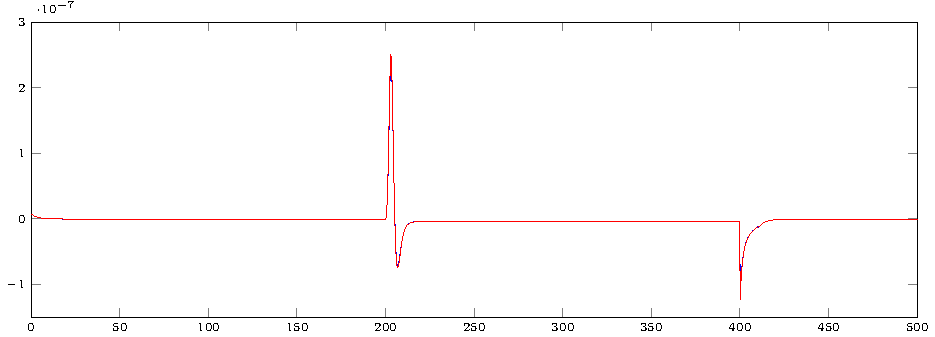
\includegraphics[width=15cm]{figures/diff_cor.pdf}
	\caption{The flux through the BK-channel in \uM m/s for the old (blue) and corrected (red) simulation }
	\label{fig:cordif}
\end{figure}
